
%% bare_conf.tex
%% V1.3
%% 2007/01/11
%% by Michael Shell
%% See:
%% http://www.michaelshell.org/
%% for current contact information.
%%
%% This is a skeleton file demonstrating the use of IEEEtran.cls
%% (requires IEEEtran.cls version 1.7 or later) with an IEEE conference paper.
%%
%% Support sites:
%% http://www.michaelshell.org/tex/ieeetran/
%% http://www.ctan.org/tex-archive/macros/latex/contrib/IEEEtran/
%% and
%% http://www.ieee.org/

%%*************************************************************************
%% Legal Notice:
%% This code is offered as-is without any warranty either expressed or
%% implied; without even the implied warranty of MERCHANTABILITY or
%% FITNESS FOR A PARTICULAR PURPOSE! 
%% User assumes all risk.
%% In no event shall IEEE or any contributor to this code be liable for
%% any damages or losses, including, but not limited to, incidental,
%% consequential, or any other damages, resulting from the use or misuse
%% of any information contained here.
%%
%% All comments are the opinions of their respective authors and are not
%% necessarily endorsed by the IEEE.
%%
%% This work is distributed under the LaTeX Project Public License (LPPL)
%% ( http://www.latex-project.org/ ) version 1.3, and may be freely used,
%% distributed and modified. A copy of the LPPL, version 1.3, is included
%% in the base LaTeX documentation of all distributions of LaTeX released
%% 2003/12/01 or later.
%% Retain all contribution notices and credits.
%% ** Modified files should be clearly indicated as such, including  **
%% ** renaming them and changing author support contact information. **
%%
%% File list of work: IEEEtran.cls, IEEEtran_HOWTO.pdf, bare_adv.tex,
%%                    bare_conf.tex, bare_jrnl.tex, bare_jrnl_compsoc.tex
%%*************************************************************************
%

\documentclass[conference]{IEEEtran}

\usepackage{graphicx}
\usepackage{color}
\usepackage{multirow}
\usepackage{placeins}
\usepackage{mdwmath}
\usepackage{balance}
\usepackage{amsmath}
%\usepackage{flushend}
\newcommand \todo[1]{\textcolor{red}{\textsl{TODO: }}{\textcolor{black}{#1}}}
\newcommand \modified[1]{{\textcolor{black}{#1}}}
\hyphenation{op-tical net-works semi-conduc-tor}

\begin{document}
\title{White Rabbit Transparent Clock}
% author names and affiliations
% use a multiple column layout for up to three different
% affiliations
% 
% conference papers do not typically use \thanks and this command
% is locked out in conference mode. If really needed, such as for
% the acknowledgment of grants, issue a \IEEEoverridecommandlockouts
% after \documentclass

% for over three affiliations, or if they all won't fit within the width
% of the page, use this alternative format:
% 
\author{\IEEEauthorblockN{Cesar Prados\IEEEauthorrefmark{1}
\IEEEauthorrefmark{3}}
\IEEEauthorblockA{\IEEEauthorrefmark{1}GSI,Darmstadt Germany}
\IEEEauthorblockA{\IEEEauthorrefmark{3}Technical University Darmstadt, Darmstadt Germany}
}


\maketitle

\begin{abstract}
 A new timing system based on White Rabbit (WR) is being developed for the
 upcoming FAIR facility at GSI, in collaboration with CERN, other institutes and
 industry partners. The timing system is responsible for the synchronization of
 nodes with nanosecond accuracy and distribution of timing messages, which
 allows for real-time control of the accelerator equipment. WR is a fully
 deterministic Ethernet-based network for general data transfer and
 synchronization, which is based on Synchronous Ethernet and PTP. The ongoing
 development at GSI aims for a miniature timing system, which is part of a
 control system of a proton source, that will be used at one of the accelerators
 at FAIR. Such a timing system consists of a Data Master generating timing
 messages, which are forwarded by a WR switch to a handful of timing receivers.
 The next step is an enhancement of the robustness, reliability and scalability
 of the system. These features will be integrated in the forthcoming CRYRING
 control system in GSI. CRYRING serves as a prototype and testing ground for the
 final control system for FAIR. The contribution presents the overall design and
 status of the timing system development.
\end{abstract}




\section{INTRODUCTION}

The GMT triggers and synchronizes accelerator equipment accordingly 
to the accelerator cycles~\cite{fair_rep}. Cycle lengths range 
from 20 ms (present UNILAC), several seconds (synchrotrons SIS18 
and SIS100/300) to several hours (storage rings). The beam production chain is an important concept in
accelerator control systems. It describes the production of a beam
from an ion source through the accelerators to a target. Properties of such a beam production 
chain include the ion type (from protons to uranium), energy, intensity, focus
and emittance at the final destination and other parameters. This information is
conveyed to the GMT, which 
has an integral view on the tightly synchronized accelerators and beam transfer
sections. The GMT must take into account the execution of several beam production 
chains in the accelerator complex at the same time. For each part of the machine, switching 
between different beam production chains will be possible between cycles, which implies a 
high degree of true parallel operation.

The GTM is made of an interconnected network of Timing Receiver Nodes (TRN) and
special nodes so-called Masters. The TRN are devices synchronized to the Timing
Master, source of time and frequency for all the network, and they are also the
receivers of timing events from the Data Master. The interconnection is
established using WR Switches, which are responsible of the propagation of the
synchronization and timing events to the TRN.



\section{White Rabbit PTP}
\label{sec:wr}

%\subsection{White Rabbit Synchronization}
WR reaches sub-nanosecond synchronization with picosecond jitter, basically, 
characterizing the asymmetries of the link, and using a clock loopback
technique for tracking the phase shift between the master reference clock
signal and the clock signal of the slave. In order to gather and
accomplish such a measurement WR extends PTP, WRPTP~\cite{biblio:ispcs_m}. 
\figurename~\ref{fig:wr_ptp} shows the WRPTP flow of messages and the
integration with standard PTP once is established.

Below is the summary of the steps, measurement and hardware support needed for the 
WR synchronization between two WR devices. A thorough description is presented 
in ~\cite{biblio:tomas} and ~\cite{biblio:wrptp}.

\subsubsection{WR Discovery and Syntonization}

A WR clock initiates WRPTP with an announcement message in order to discover
other WR devices. If a WR device has been discovered, the master will initiate the 
frequency lock procedure. WRPTP uses SyncE to distribute a common frequency throughout 
the network, the WR Slaves are frequency locked to the WR Master. 

\subsubsection{Asymmetry Calibration}

Once the slave is locked to the master, the WR devices initiate to calibrate the 
asymmetries in the common optical link taking in consideration:

\begin{itemize}
    \item Fixed delays due to transmission circuitry
    \item Asymmetry of the optical transceivers and PHYs 
    \item Asymmetry of the propagation delay in the fiber caused by the chromatic dispersion
\end{itemize}

\subsubsection{Coarse and Fine Delay Measurement}
\label{sec:delay_ms}
After the devices are calibrated, a first delay measurement, \textit{Coarse
Measurement}, is issued using the delay request-respond (DRR) mechanism. 
The next step towards the synchronization requires the measurement of the phase shift
between a reference (master) clock signal and the loopback clock signal
of the slave. For this purpose, WR implements Digital Dual Mixer Time Difference
(DDMTD) ~\cite{biblio:ddmtd} phase detection. The DDMTD measures the \textit{round trip phase
shift}, $phase_{mm}$.

With the $phase_{mm}$, the delay round trip, $delay_{mm}$ is calculated. The $phase_{s}$
is the phase shift of the clock adjustment (see \figurename~\ref{fig:wr_time_stamp})  
derived from the $offset_{ms}$. Using the $phase_{mm}$ and $phase_{s}$, 
the timestamps on ingress ports can be enhanced,
$t_{2p}$ and  $t_{4p}$, using a decision algorithm described in ~\cite{biblio:tomas}.
Only timestamps on ingress ports need to be enhanced, since they are generated 
asynchronously to the reference clock domain. The \textit{Fine Delay Measurement}, round trip,
is calculated as follows, using the enhanced timestamps :

\begin{equation}
  \label{eq:round_trip}
    delay_{mm} = (t_{4p} - t_1) - (t_3 - t_{2p})
\end{equation}

\figurename~\ref{fig:wr_ptp} shows how after the initial WRPTP synchronization, 
a DRR or peer delay (PD) mechanism produces the timestamps, $t_{1}$, $t_{2p}$,
$t_{3}$ and $t_{4p}$ (in the case of PD, also
$t_{5}$ and $t_{6p})$.

\subsubsection{Synchronization}
In order to finish the synchronization, the offset between both clocks must be
calculated, $offset_{ms}$. 
The round trip can be expressed as a function of the  delay master to slave, $\sigma _{ms}$ , slave to
master $\sigma _{sm}$ and the sum of the fixed delays, $\Delta$ , obtained during the calibration.

\begin{equation}
  \label{eq:round_trip_2}
    delay_{mm} = \Delta + \sigma _{ms} + \sigma _{sm}
\end{equation}

The ratio between single delays is proportional to the asymmetry of the speed of
the different wavelengths due to the chromatic dispersion in the fiber optic
link:

\begin{equation}
    \label{eq:disp}
    (\alpha-1) = \frac{\sigma_{ms}}{\sigma_{sm}}
\end{equation}

\begin{figure}[!t]
\centering
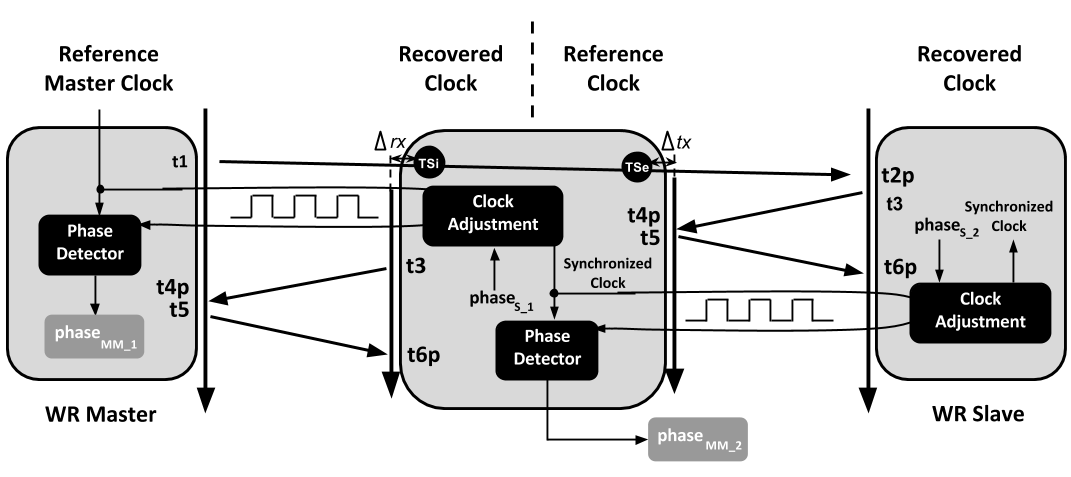
\includegraphics[scale=0.26]{fig/time_stamps_tc.png}
\caption{WR Loopback Clock, Phase Detection and Enhanced Time Stamps}
\label{fig:wr_time_stamp}
\end{figure}


Combining equations (\ref{eq:round_trip}), (\ref{eq:round_trip_2}) and
(\ref{eq:disp}), the delay master to slave and $offset_{MS}$:

\begin{equation}
    \label{eq:delayms}
     delay_{ms} = \frac{1+ \alpha}{2+ \alpha}(delay_{mm} - \Delta)+ \Delta_{txm} + \Delta_{rxs} 
\end{equation}

\begin{equation}
    \label{eq:offsetms}
    offset_{ms} = t_{1} - t_{2p} - delay_{ms}
\end{equation}

\begin{figure}[!t]
\centering
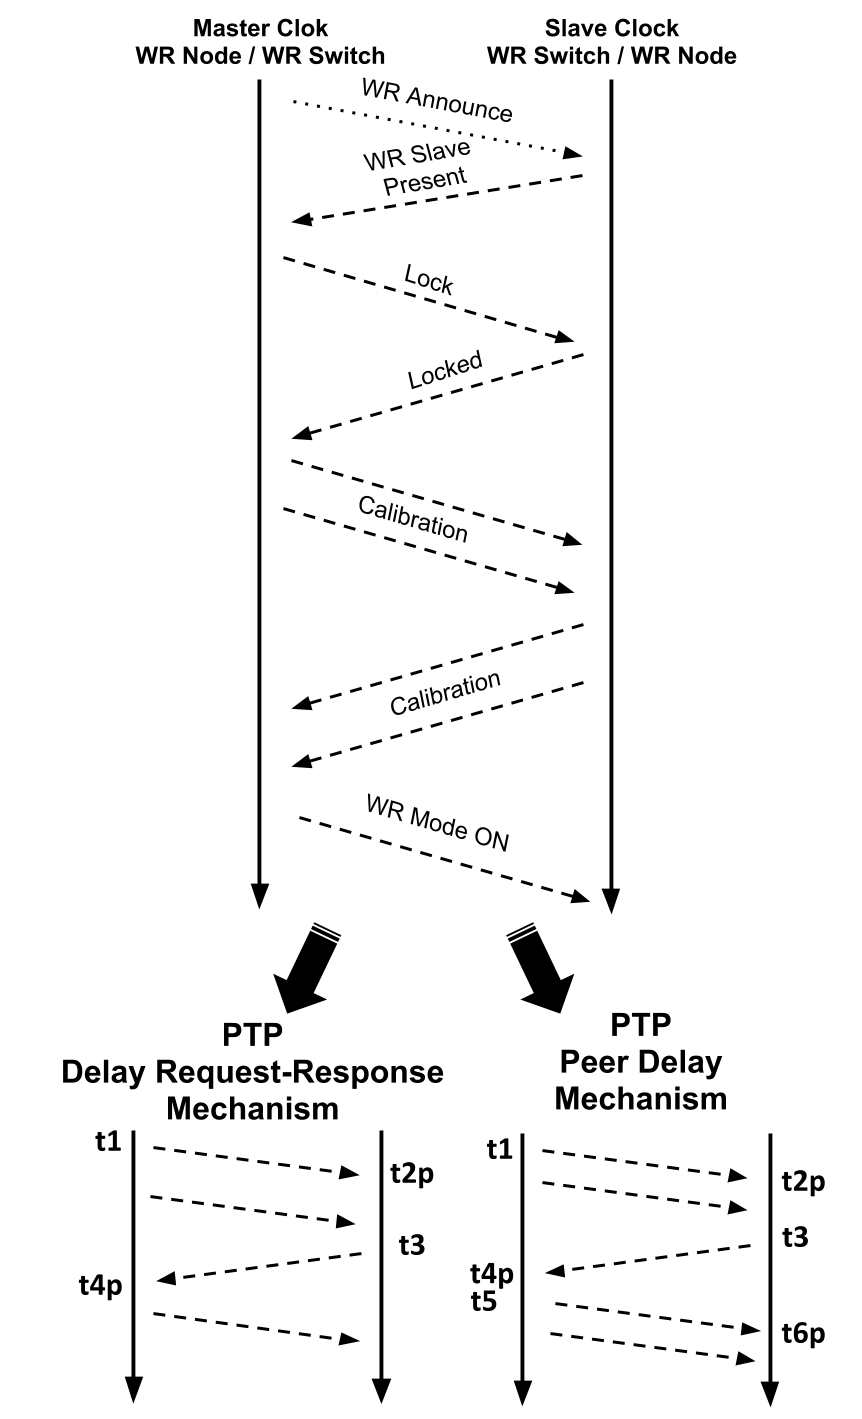
\includegraphics[scale=0.25]{fig/wr_ptp.png}
\caption{WR PTP Message Flow and PTP}
\label{fig:wr_ptp}
\end{figure}




\section{WR Transparent Clocks}
\label{sec:wr_tc}
PTP Transparent Clock (TC) modifies PTP messages as they pass through them
adding the residence time to an accumulative Correction Field (CF) in the PTP 
messages. Thus, the delay introduced  by the network is measured and can be 
subtracted in the slave clock, which improves distribution accuracy.

In ~\ref{sec:wr} the WRPTP and WR synchronization steps have been described for
master, slave and boundary clocks. This chapter presents how a standard TC becomes a WR TC.

\begin{figure*}[!t]
\centering
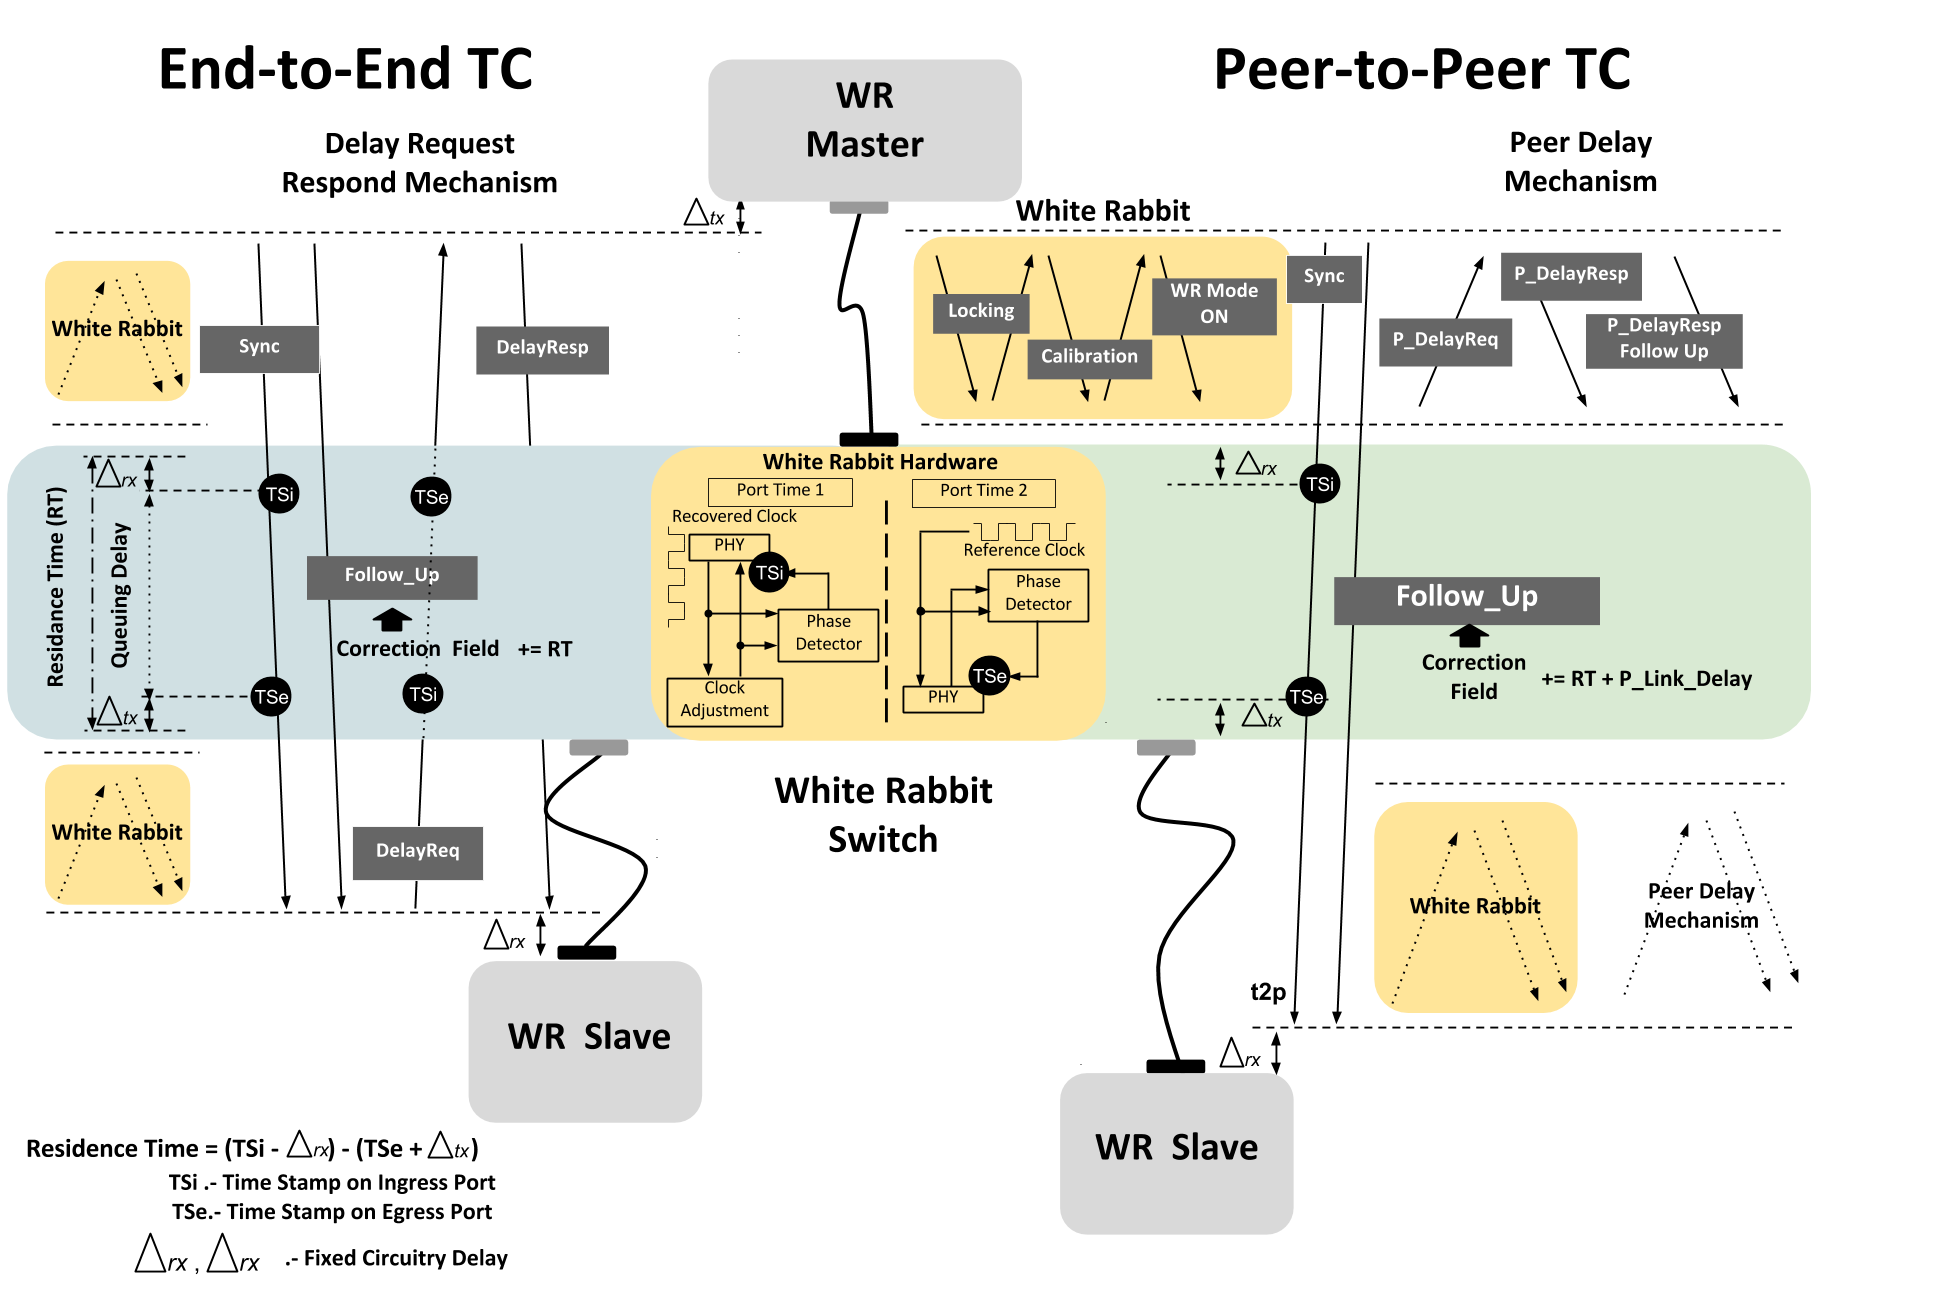
\includegraphics[scale=0.27]{fig/wr_schema_hw_bw.png}
\caption{WR End two End and Peer to Peer Transparent Clocks}
\label{fig:wr_tc}
\end{figure*}

%\subsection{End-to-End WR Transparent Clock}
%
%As the standard End-to-End (E2E) clocks, the WR E2E TC doesn't belong to the
%master-slave hierarchy and does not synchronized to the WR Master. 
%Therefore, a WR E2E accomplishes only the synthonization and the calibration.
%Thus the WR Mode is on without the $phase_{mm}$ or $phase_{s}$ measurement
%between the master and the slave, but between the slave and the adjacent WR
%Switch. 
%
%The \figurename~\ref{fig:wr_tc} shows the PTP exchange of messages from master to slave,
%going through the switch transparently and how the residence time is also calculated taking into 
%account the fixed delays $\Delta$. Thanks to the synthonization and fixed delay measurements done during 
%the WRPTP there is not error in the measurement of the residence time. A two-step WR E2E TC calculates, using
%(\ref{eq:delayms}), the $offset_{ms}$:
%
%\begin{equation}
%    \label{eq:residence_time}
%     CF += (TS_{ingess\_port} - \Delta_{rx}) -
%     (TS_{egress\_port} + \Delta_{tx})
%\end{equation}
%
%\begin{equation}
%    \label{eq:wre2e}
%     offset_{ms} = t_{1} - t_{2} - delay_{ms} - CF
%\end{equation}
%
\subsection*{Peer-to-Peer WR Transparent Clock}

As the standard Peer-to-Peer (P2P) clocks, the WR P2P TC measures residence time
of Sync messages, and the link delay in both directions. The
\figurename~\ref{fig:wr_time_stamp} and \figurename~\ref{fig:wr_tc}
show the PTP exchange of messages from master to slave going through the switch 
transparently and how the residence time is also calculated taking into  account the fixed delays $\Delta$. 


The link delay between master and slave is calculated according to~\eqref{eq:round_trip_2}:

\begin{equation}
  \label{eq:delayss_1}
    delay_{ss} = \Delta + \sigma _{ms} + \sigma _{sm}
\end{equation}

using the fiber asymmetry relation~\eqref{eq:disp}:

\begin{equation}
  \label{eq:delayss_2}
    delay_{ss} = \Delta + (1 + \alpha) \sigma _{sm} + \sigma _{sm}
\end{equation}

adding the fixed delays due to transmission circuitry:

\begin{equation}
    \label{eq:delaysm}
     delay_{sm} = \frac{delay_{ss} - \Delta}{2+ \alpha} + \Delta_{txs} +
     \Delta_{rxm} 
\end{equation}

Since the link delay is done between adjacent clocks using the peer delay mechanism, 
the full WR synchronization process can be issued between the two ports. 
The measurement of the residence time, like in the BC should suffer no error
since the ports are syntonized to its master clock, but also the measurement of the
link delays, are as precise as the WR project claims ~\cite{biblio:ispcs_m} for the
Boundary Clocks. The link delay is calculated like in \eqref{eq:delayms}, 
but using $t_{3}$, $t_{4p}$, $t_{5}$ and $t_{6p}$ instead. The $offset_{ms}$ is calculated:

\begin{equation}
    \label{eq:residence_time}
     residence\_time= (TS_{ingess\_port} - \Delta_{rx}) -
     (TS_{egress\_port} + \Delta_{tx})
\end{equation}


\begin{equation}
    \label{eq:wrp2p}
     CF += residance\_time + delay\_link
\end{equation}


\begin{equation}
    \label{eq:wrp2p_1}
     offset_{ms}= t_{1} - t_{2} - CF - delay\_link \footnote{This link delay
     corresponds to the last link to the slave}
\end{equation}

%\FloatBarrier


\section{Performance of WR Transparent Clocks}
\label{sec:issues}
This section examines the features of WR TC that are commonly~\cite{biblio:tc_perf} taken in to
account for the estimation of the performance of a TC: 
\begin{itemize}
    \item Accuracy and precision
    \item Correction factor stability
    \item Maximum update rate
    \item Rapid reconfiguration after topology changes
\end{itemize}


\subsection{Accuracy and precision}

%\subsubsection{WR TC Peer to Peer}
%The chapter ~\ref{sec:wr} resumes how WR accomplish
%sub-nanoseconds synchronization and picoseconds jitter. It is based on the
%acharacterization the asymmetries of the link a priory, and a clock lookback
%technique. By doing this WR is able to  enhance the timestamps on ingress ports. 

The performance of the WR Peer-to-Peer TC prototype is compared in this section
with the WR BC. For this purpose, the pulse per second (PPS) skew between a WR slave clock 
connected to a WR master clock using up to 5 WR switches is measured.
\figurename~\ref{fig:test_setup} shows the setup used for the benchmarking. 
The WR master and slave clocks are Exploder cards
~\cite{biblio:wr_gsi} with a modified WR PTP software~\cite{biblio:wrpc-sw}.
The switches are WR v3 with a modified firmware. The WR master and slave
are connected to a Lecroy Waverunner oscilloscope using lemo cables of the 
same length. 

The histograms in \figurename~\ref{fig:wr_bc} and~\ref{fig:wr_p2p} show the outcome of the
measurements.

%\subsubsection{WR TC End to End}
%\begin{figure}[!t]
%%\centering
%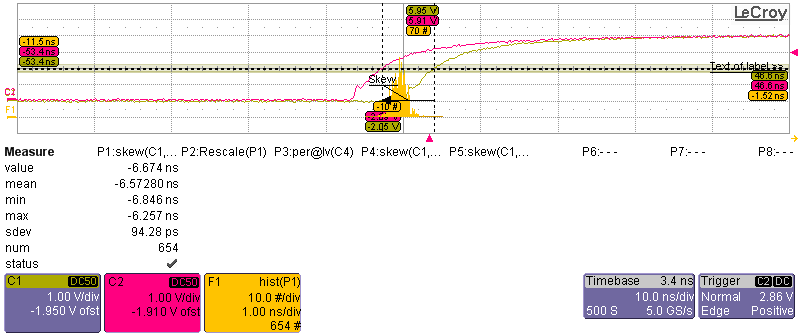
\includegraphics[scale=0.25]{fig/tc_5_switches2.png}
%\caption{WR E2E and P2P Transparent Clocks}
%\label{fig:wr_tc}
%\end{figure}
%
The offset between master and slave is in the range of nanoseconds and
increases with the number of switches in cascade. Since the WR nodes~\cite{biblio:wr_gsi} 
and small form-factor pluggable (SFP) used in this setup haven't been calibrated yet, 
the fixed delays are missing in the
calculation of $delay_{ms}$~\eqref{eq:delayms}. In the case of the TC also
affects to the measurement of the residence time~\eqref{eq:residence_time}. This
explains the difference of almost 1 ns offset between the clocks, as well as
the increment of the offset as the number of TCs in the topology increases.

The standard deviation, $\delta^2$, of the PPS skew in the TC is almost constant, 
while in the BC increases as the number of BC increases. 
This result shows that the WR model is also applicable to TC even though the
phase measurement and the time stamp enhancement~\ref{sec:delay_ms} is not done between master and
slave clock, but between TCs or slaves. 

\FloatBarrier
\begin{figure}[!t]
\centering
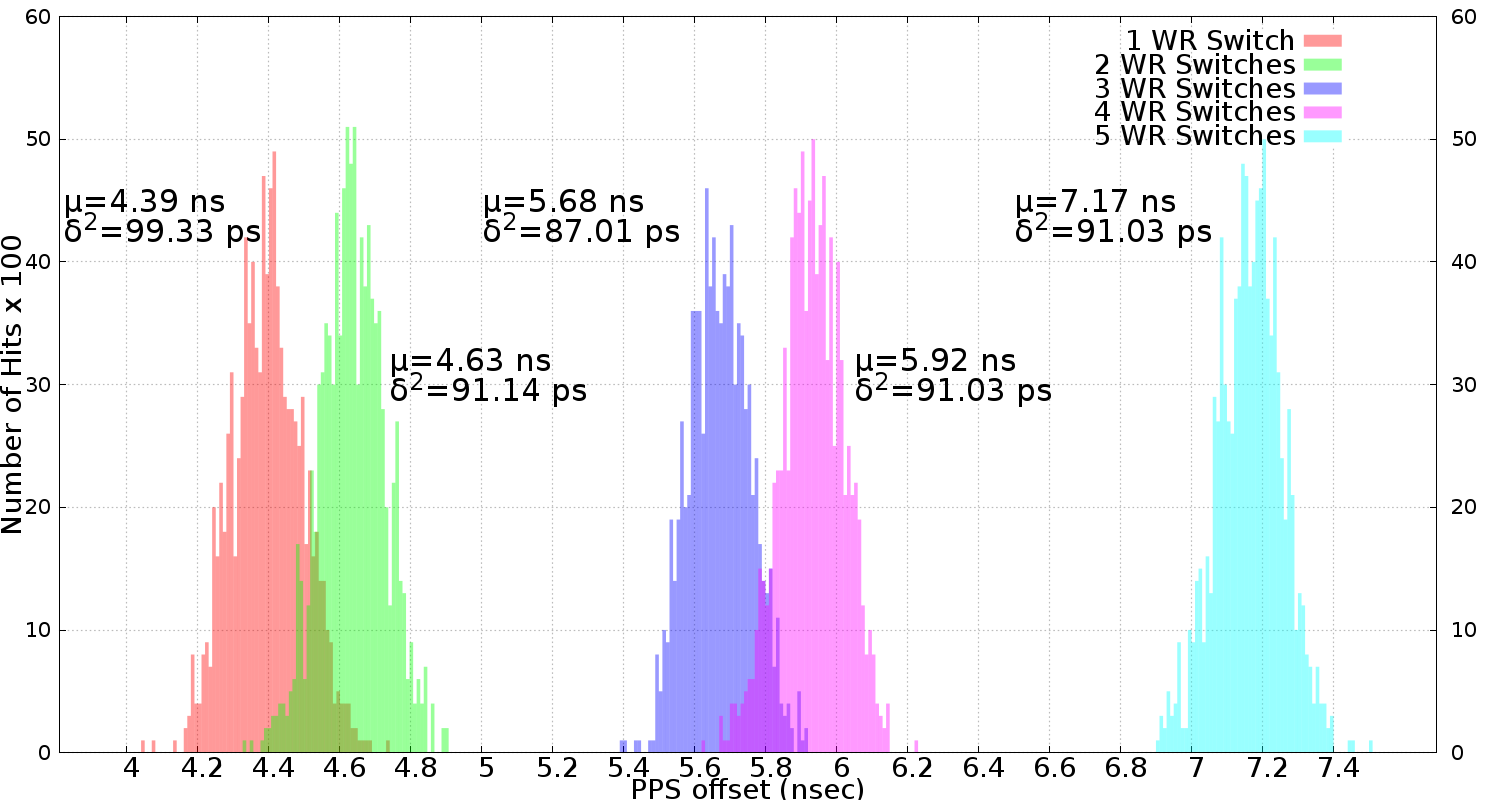
\includegraphics[scale=0.29]{fig/p2p.png}
\caption{Histogram of PPS offset between WR Master, up to 5 WR TC Peer-to-Peer and WR Slave}
\label{fig:wr_p2p}
\end{figure}

\subsection{Residence Time Stability and Maximum Update Rate}

Both, maximum update rate and residence time, are features greatly influenced
by the latency in the TCs. As a result, the synchronization could suffer
performance degradation. 

An increment of the residence time in a TC is normally associated 
to an increment of the traffic in the switch. The authors of ~\cite{biblio:tc_perf} 
present the parameter \textit{Correction Factor Error} (CFE). It expresses the difference 
of the latency measured by a test equipment and TC under test. The origin of this error in 
the measurement of the residence time is implementation-dependent, and it can be associated 
in the most of the cases with delays in the input or output queues of the switch.

During the acquisition of measurements for this paper, the residence time in the
WR TCs has been constant. The propagation delay from master to slave 
minus the residence time in every TC, has only varied in the range of
picosecond in successive samplings. The reason lies in the design of the
hardware in charge of the timestamping~\cite{biblio:tomas} and
deterministic packet forwarding. The WR switch generates the timestamps after 
the output queues. Thereby, the non deterministic delay
introduced during the queuing is already measured in the residence time and the
CFE should be negligible. Besides that, WR switches provide deterministic packet forwarding making use of a 
quality of service (QoS) prioritization scheme and cut-through
switching~\cite{biblio:switch_book}. The traffic tagged as highest priority will be forwarded 
without a maximum delay. The rest of the traffic will follow a queue scheduling algorithm and
store and forward switching~\cite{biblio:switch_book}.

The \textit{Update Rate} (UR) of a two-step clock, is defined as the delay between the transmission of a Sync
message from the master till the reception of the Follow Up message by the slave. 
According to~\cite{biblio:tc_perf}, delays around $10-30\%$ of the Sync interval can create
instability in the slave. 

\FloatBarrier
\begin{figure}[!t]
\centering
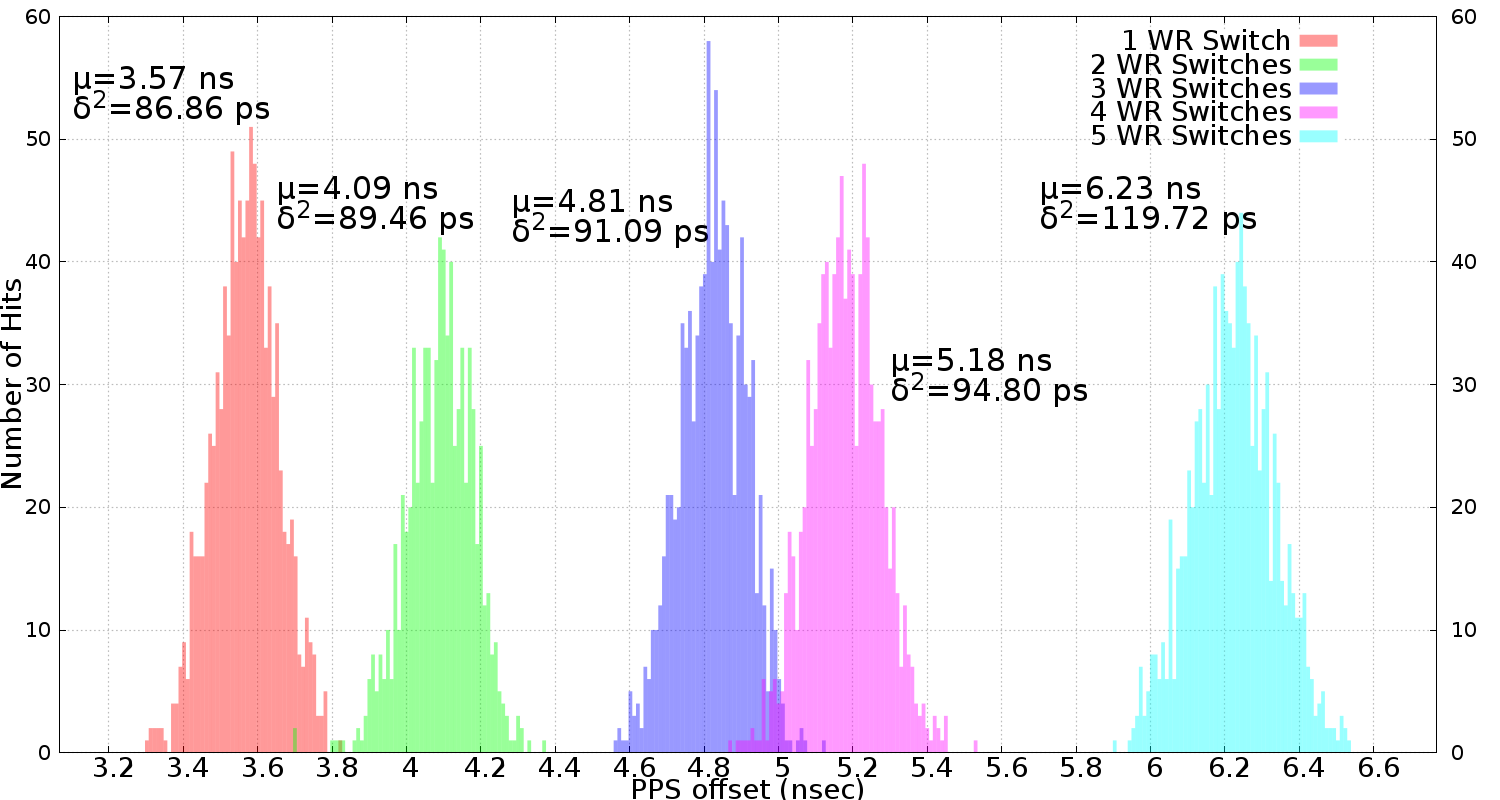
\includegraphics[scale=0.29]{fig/bc.png}
\caption{Histogram of PPS offset between WR Master, up to 5 WR BC and WR Slave}
\label{fig:wr_bc}
\end{figure}

\figurename~\ref{fig:update_rate} shows the average, maximum and minimum delay between SYNC
transmission and FOLLOW\_UP reception in topologies up to 5 layers of TC. Since
the processing of the Sync packets flow, in WR TC, is done in software, the
delay is in the range of milliseconds, and the ratio between the UR and the
SYNC rate, $1 Hz$, is between $10-20\%$. Despite that, the measurements in
\figurename~\ref{fig:wr_p2p}, show a stable and tight synchronization of the
slaves to the master.

\FloatBarrier
\begin{figure}[!t]
\centering
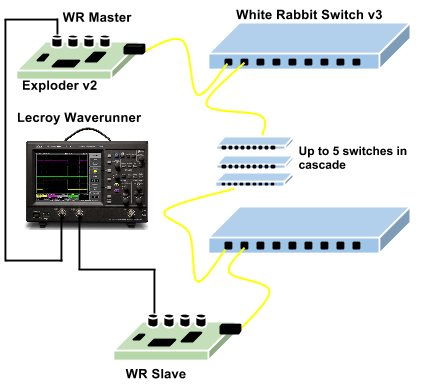
\includegraphics[scale=0.50]{fig/tc_test_bed.png}
\caption{Test setup}
\label{fig:test_setup}
\end{figure}


\subsection{Reconfiguration after Topologies Changes}

A timing system application, often, demands not only accuracy and precision, 
but also stability and continuation of the synchronization in the events
of failure. As an illustrative example, the new timing systems for GSI and CERN,
based on WR technology, require a high stability of the synchronization. 
Both timing systems achieve resilience against 
network failures using redundant connections.  Lower layer protocols stablish a
spanning tree topology setting ports connected to cyclic paths to block/passive
state. In this case only the Peer-to-Peer TC still issues the synchronization between the
ports in both directions. As a result, both clocks have the link delay
information. This offers the possibility of having the link immediately available after 
changes in the topology. Hence the reconfiguration time doesn't depend on the TCs anymore 
but in the lower layer protocol. WRS has already
proposals for implementing a transparent mechanism ~\cite{biblio:wrswitch} for
recovering from single points of failure in a redundant network.

\begin{figure}[!t]
\centering
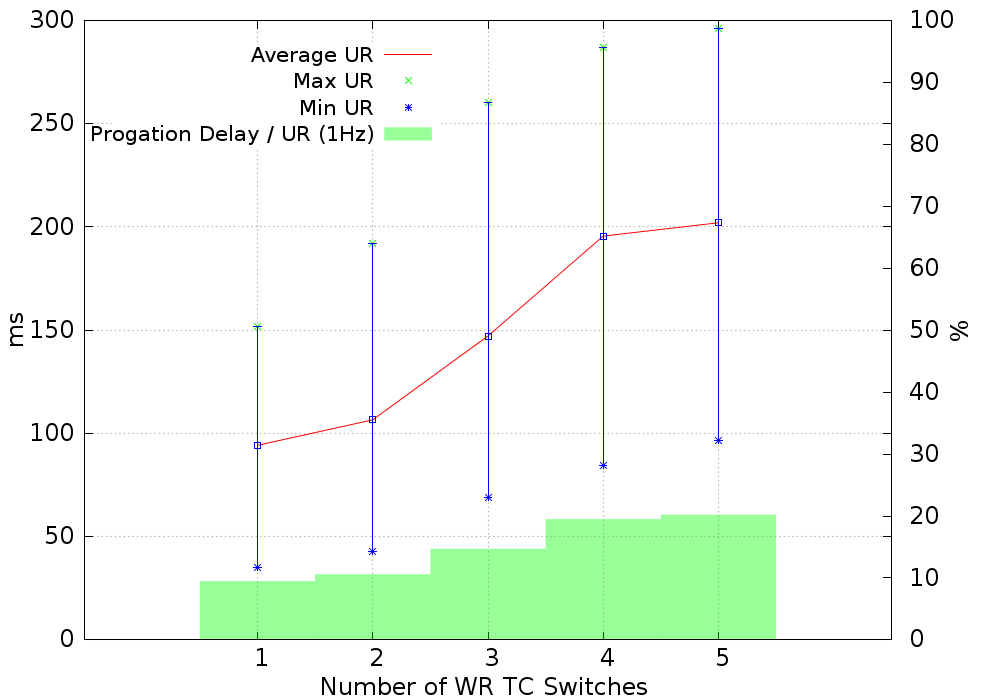
\includegraphics[scale=0.27]{fig/update_rate.png}
\caption{SYNC transmission to FOLLOW\_UP reception delay and Update Rate}
\label{fig:update_rate}
\end{figure}


\section{Conclusion and Future Work}
This paper demonstrates that the WR hardware and mechanism can be used 
successfully in a TC. The measurements point out a slightly better performance
of the WR TCs in terms of standard deviation of the PPS skew, 
and despite the large delays introduced by the software during the forwarding of 
the SYNC packets, the synchronization is highly stable. 

Altogether, the WR Peer-to-Peer TCs are suitable for timing systems with 
demanding requirements in terms of reliability, in addition to the
sub-nanosecond synchronization. Therefore the test presented in the paper will
be carried out again with the correct calibration values. In addition, 
the author has already begun to study the synchronization resilience of systems 
based on TCs and lower layer protocols for recovering from network failures. 



%\section{Acknowledgment}
The Author would like to recognize the vast work done by the WR Community 
and specially to, T. W\l{}ostowski and M. Lipiński, for their support,  
design and code of the White Rabbit Switch, on which this paper is based.




\bibliographystyle{IEEEtran}
\balance
\bibliography{IEEEabrv,./biblio}

\end{document}


